\subsection{Bài tập trắc nghiệm cuối bài}
\TN
\setcounter{ex}{0}
\Opensolutionfile{ans}[ans/1D1-B3-1]
\begin{ex}%[1D1Y1]
	Tập giá trị của hàm số $y= \cos x$ là tập hợp nào sau đây?
	\choice
	{$\mathbb{R}$}
	{$(-\infty; 0]$}
	{$[0; +\infty]$}
	{\True $ [-1; 1]$}
	\loigiai{
		Với mọi $x \in \mathbb{R}$ thì $-1 \leq \cos x \leq 1$. 
	}
\end{ex}

\begin{ex}%[1D1Y1]
	Tập giá trị của hàm số $y=\sin 2x$ là
	\choice{$[-2;2]$}
	{$[0;2]$}
	{\True $[-1;1]$}
	{$[0;1]$}
	\loigiai{
		Tập giá trị của hàm số $y=\sin 2x$ là $[-1;1]$}
\end{ex}

\begin{ex}%[1D1B1]
	Mệnh đề nào dưới đây \textbf{sai}?
	\choice
	{Hàm số $y=\tan x$ tuần hoàn với chu kì $\pi$}
	{\True Hàm số $y=\cos x$ tuần hoàn với chu kì $\pi$}
	{Hàm số $y=\cot x$ tuần hoàn với chu kì $\pi$}
	{Hàm số $y=\sin2x$ tuần hoàn với chu kì $\pi$}
	\loigiai{
		Hàm số $y=\cos x$ tuần hoàn với chu kì $2\pi$, các hàm số $y=\tan x, y=\cot x, y=\sin2x$ tuần hoàn với chu kì $\pi$.
	}
\end{ex}

\begin{ex}%[1D1B1]
	Hàm số $y=\sin 2x$ có chu kỳ tuần hoàn là
	\choice
	{$T=2\pi$}
	{$T=\dfrac{\pi}{2}$}
	{\True $T=\pi$}
	{$T=4\pi$}
	\loigiai{ 
		Chú ý với $k$ là số nguyên dương hàm số $y=\sin kx$ có chu kỳ $T= \dfrac{2\pi}{k}$. 
	}
\end{ex}

\begin{ex}%[1D1Y1]
	Mệnh đề nào dưới đây đúng?
	\choice
	{Hàm số $y=\sin x$ là hàm số chẵn}
	{\True Hàm số $y=\cos x$ là hàm số chẵn}
	{Hàm số $y=\tan x$ là hàm số chẵn}
	{Hàm số $y=\cot x$ là hàm số chẵn}
	\loigiai{
		Theo định nghĩa thì trong bốn hàm số đã cho, chỉ có hàm số $y=\cos x$ là hàm số chẵn.
	}
\end{ex}

\begin{ex}%[1D1Y1]
	Tìm hàm số lẻ trong các hàm số sau:
	\choice
	{$y=\sin^2x$}
	{\True $y=x\cos2x$}
	{ $y=x\sin x$}
	{$y=\cos x$}	
	\loigiai{
		Tất cả các hàm ở 4 đáp án đều có tập xác định là $\mathbb{R}$,  nên để kiểm tra tính lẻ, ta chỉ cần kiểm tra tính chất $f(-x)$ có bằng với $f(x), \forall x\in \mathbb {R}$ và hàm đó là $y=x\cos2x$.
		
	}
	
\end{ex}

\begin{ex}%[1D1B1-3]
	Hàm số nào trong các hàm số dưới đây là hàm số chẵn?
	\choice
	{\True $y=\sin\left(x+\dfrac{\pi}{2}\right)$}
	{$y=\cos\left(x+\dfrac{\pi}{2}\right)$}
	{$y=\sin 2x$}
	{$y=\tan x-\sin 2x$}
	\loigiai{
		Xét $y=\sin\left(x+\dfrac{\pi}{2}\right)$ có tập xác định $\mathscr{D}=\mathbb{R}$.\\
		Mặt khác $y=\sin\left(x+\dfrac{\pi}{2}\right)=\cos x$ nên là hàm chẵn.
	}
\end{ex}

\begin{ex}%[1D1Y1]
	Tìm tập xác định của hàm số $ y = \cot x $.
	\choice
	{$ \mathscr D = \mathbb{R} \backslash \left\lbrace k\dfrac{\pi}{2} | k \in \mathbb{Z} \right\rbrace $}
	{\True $ \mathscr D = \mathbb{R} \backslash \{k\pi | k \in \mathbb{Z} \} $}
	{$ \mathscr D = \mathbb{R} \backslash \{k2\pi | k \in \mathbb{Z} \} $}
	{$ \mathscr D = \mathbb{R} \backslash \left\lbrace\dfrac{\pi}{2} + k \pi  | k \in \mathbb{Z} \right\rbrace $}
	\loigiai
	{
		Hàm số xác định khi và chỉ khi $\sin x \ne 0 \Leftrightarrow x \ne k \pi, k \in \mathbb{Z}.$\\
		Vậy $ \mathscr D = \mathbb{R} \backslash \{k\pi | k \in \mathbb{Z} \} $.
	}
\end{ex}

\begin{ex}%[Dương Phước Sang]%[1D1Y1-1]
	Điều kiện xác định của hàm số $y=\dfrac{1-3\cos x}{\sin x}$ là
	\choice
	{$x\ne \dfrac{\pi}{2}+k\pi,~k\in\mathbb{Z}$}
	{$x\ne k2\pi,~k\in\mathbb{Z}$}
	{$x\ne \dfrac{k\pi}{2},~k\in\mathbb{Z}$}
	{\True $x\ne k\pi,~k\in\mathbb{Z}$}
	\loigiai{
		Điều kiện xác định của hàm số đã cho là $\sin x\ne 0 \Leftrightarrow x\ne k\pi,~k\in\mathbb{Z}$.}
\end{ex}

\begin{ex}%[Dương Phước Sang]%[1D1Y1-1]
	Với ký hiệu $k\in \mathbb{Z}$, điều kiện xác định của hàm số $y=\dfrac{2\sin x+1}{1-\cos x}$ là
	\choice
	{\True $x\ne k2\pi $}
	{$x\ne k\pi $}
	{$x\ne \dfrac{\pi}{2}+k\pi $}
	{$x\ne \dfrac{\pi}{2}+k2\pi $}
	\loigiai{
		Hàm số xác định $ \Leftrightarrow 1-\cos x\ne 0 \Leftrightarrow \cos x\ne 1\Leftrightarrow x\ne k2\pi ~(k\in \mathbb{Z})$.\\
		Vậy điều kiện xác định của hàm số đã cho là $x\ne k2\pi~(k\in \mathbb{Z})$.}
\end{ex}
\begin{ex}%[Dương Phước Sang]%[1D1Y1-1]
	Với ký hiệu $k \in \mathbb{Z}$, điều kiện xác định của hàm số $y=\tan \left(2x-\dfrac{\pi}{3}\right)$ là
	\choice
	{$x\ne \dfrac{\pi}{6}+k\dfrac{\pi}{2}$}
	{$x\ne \dfrac{5\pi}{12}+k\pi $}
	{$x\ne \dfrac{\pi}{2}+k\pi $}
	{\True $x\ne \dfrac{5\pi}{12}+k\dfrac{\pi}{2}$}
	\loigiai{
		Hàm số xác định $ \Leftrightarrow \cos \left(2x-\dfrac{\pi}{3}\right)\ne 0\Leftrightarrow 2x-\dfrac{\pi}{3}\ne \dfrac{\pi}{2}+k\pi\Leftrightarrow x\ne \dfrac{5\pi}{12}+k\dfrac{\pi}{2}~(k\in \mathbb{Z})$.\\
		Vậy điều kiện xác định của hàm số đã cho là $x\ne \dfrac{5\pi}{12}+k\dfrac{\pi}{2}~(k\in \mathbb{Z})$.}
\end{ex}

\begin{ex}%[1D1B1]
	Tìm điều kiện xác định của hàm số $ y = \tan x + \cot x $.	
	\choice
	{$ x \neq k \pi, k \in \mathbb{Z} $}
	{$ x \neq \dfrac{\pi}{2} + k \pi, k \in \mathbb{Z} $}
	{\True $ x \neq \dfrac{k \pi}{2}, k \in \mathbb{Z} $}
	{$ x \in \mathbb{R} $}
	\loigiai{
		Hàm số xác định $ \Leftrightarrow \sin 2x \neq 0 \Leftrightarrow x \neq \dfrac{k \pi}{2}, k \in \mathbb{Z} $.	
	}
\end{ex}	

\begin{ex}%[1D1B1]
	Tập xác định của hàm số $y=\dfrac{2\cos 3x-1}{\cos x+1}$ là
	\choice
	{$\mathscr{D}=\mathbb{R}\setminus \{\pi+k\pi;k\in\mathbb{Z}\}$}
	{$\mathscr{D}=\mathbb{R}\setminus \{k2\pi;k\in\mathbb{Z}\}$}
	{$\mathscr{D}=\mathbb{R}\setminus \{\dfrac{\pi}{2}+k\pi;k\in\mathbb{Z}\}$}
	{\True $\mathscr{D}=\mathbb{R}\setminus \{\pi+k2\pi;k\in\mathbb{Z}\}$}
	\loigiai{Hàm số xác định khi và chỉ khi $\cos x+1\ne 0\Leftrightarrow \cos x\ne -1\Leftrightarrow x\ne \pi+k2\pi, k\in\mathbb{Z}$.\\
		Vậy hàm số có tập xác định $\mathscr{D}=\mathbb{R}\setminus \{\pi+k2\pi;k\in\mathbb{Z}\}$.}
\end{ex}

\begin{ex}%[1D1B1-5]
	Tìm giá trị lớn nhất, giá trị nhỏ nhất của hàm số sau $y=1+3\sin\left(2x-\dfrac{\pi}{4}\right)$.
	\choice
	{\True $\min y=-2$, $\max y=4$}
	{$\min y=2$, $\max y=4$}
	{$\min y=-2$, $\max y=3$}
	{$\min y=-1$, $\max y=4$}
	\loigiai{Ta có: $-1\le\sin\left(2x-\dfrac{\pi}{4}\right)\le 1\Rightarrow -2\le y\le 4$.
		\begin{itemize}
			\item $y=-2\Leftrightarrow \sin\left(2x-\dfrac{\pi}{4}\right)=-1\Leftrightarrow x=-\dfrac{\pi}{8}+k\pi\Rightarrow \min y=-2$.
			\item $y=4\Leftrightarrow \sin\left(2x-\dfrac{\pi}{4}\right)=1\Leftrightarrow x=\dfrac{3\pi}{8}+k\pi\Rightarrow \max y=4$.
	\end{itemize}}
\end{ex}

\begin{ex}%[1D1B1-5]
	Tìm giá trị lớn nhất, giá trị nhỏ nhất của hàm số sau $y=3-2\cos^23x$.
	\choice
	{$\min y=1$, $\max y=2$}
	{\True $\min y=1$, $\max y=3$}
	{$\min y=2$, $\max y=3$}
	{$\min y=-1$, $\max y=3$}
	\loigiai{Ta có: $0\le\cos^23x\le 1\Rightarrow 1\le y\le 3$.
		\begin{itemize}
			\item $y=1\Leftrightarrow \cos^23x=1\Leftrightarrow x=\dfrac{k\pi}{3}\Rightarrow \min y=1$.
			\item $y=3\Leftrightarrow \cos^23x=0\Leftrightarrow x=\dfrac{\pi}{6}+\dfrac{k\pi}{3}\Rightarrow \max y=3$.
	\end{itemize}}
\end{ex}


\begin{ex}%[1D1B1-5]
	Tìm giá trị lớn nhất, giá trị nhỏ nhất của hàm số sau $y=\sqrt{2\sin x+3}$.
	\choice
	{\True $\max y=\sqrt{5}$, $\min y=1$}
	{$\max y=\sqrt{5}$, $\min y=2\sqrt{5}$}
	{$\max y=\sqrt{5}$, $\min y=2$}
	{$\max y=\sqrt{5}$, $\min y=3$}
	\loigiai{Ta có $1\le 2\sin x+3\le 5\Rightarrow 1\le y\le \sqrt{5}$.\\
		Vậy $\max y=\sqrt{5}$ khi $\sin x=1\Leftrightarrow x=\dfrac{\pi}{2}+k2\pi$ và $\min y=1$ khi $x=-\dfrac{\pi}{2}+k2\pi$.}
\end{ex}

\begin{ex}%[1D1B1-5]
	Tìm giá trị lớn nhất, giá trị nhỏ nhất của hàm số sau $y=\dfrac{4}{1+2{\sin}^2x}$.
	\choice
	{\True $\min y=\dfrac{4}{3}$, $\max y=4$}
	{$\min y=\dfrac{4}{3}$, $\max y=3$}
	{$\min y=\dfrac{4}{3}$, $\max y=2$}
	{$\min y=\dfrac{1}{2}$, $\max y=4$}
	\loigiai{
		Ta có: $0\le \sin^2x\le 1\Rightarrow \dfrac{4}{3}\le y\le 4$.
		\begin{itemize}
			\item $y=\dfrac{4}{3}\Leftrightarrow \sin^2x=1\Leftrightarrow x=\dfrac{\pi}{2}+k\pi\Rightarrow \min y=\dfrac{4}{3}$.
			\item $y=4\Leftrightarrow \sin^2x=0\Leftrightarrow x=k\pi\Rightarrow \max y=4$.
	\end{itemize}}
\end{ex}

\begin{ex}%[1D1Y1]
	Đường cong trong hình dưới đây là đồ thị của một hàm số trong bốn hàm số được liệt kê ở bốn phương án A,B,C,D. Hỏi hàm số đó là hàm số nào?
	\begin{center}
		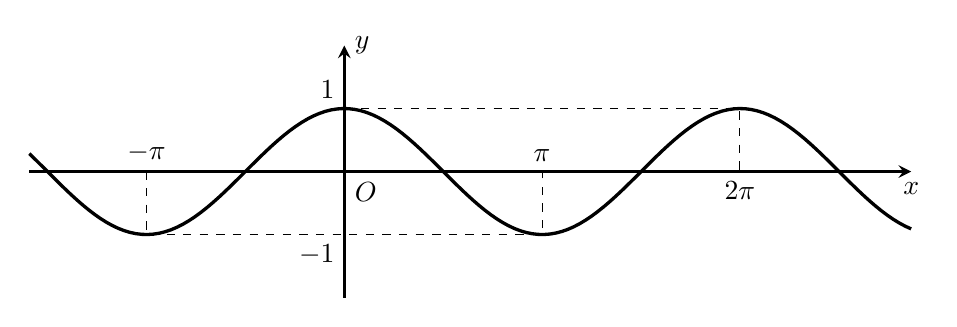
\begin{tikzpicture}[>=stealth,scale=0.8]
			\draw[->, line width = 1pt] (-5,0)-- (0,0) node [below right]{$O$}--(9,0) node[below]{$x$};
			\draw[->, line width = 1pt] (0,-2)--(0,2) node [right]{$y$};
			\draw (-3.14,0) node [above]{$-\pi$} (3.14,0) node [above]{$\pi$} (6.28,0) node [below]{$2\pi$};
			\draw (0,1) node [above left]{$1$};
			\draw (0,-1) node [below left]{$-1$};
			\draw [line width = 1.2pt, domain = -5:9, samples=150] plot (\x,{cos(\x*180/pi)});
			\draw [dashed] (-3.14,0)-- (-3.14,-1)-- (3.14,-1)-- (3.14,0);
			\draw [dashed] (0,1)-- (6.28,1)-- (6.28,0);
		\end{tikzpicture}
	\end{center}
	\choice{$y = 1 + \sin x$}{$y = 1 - \sin x$}{$y = \sin x$}{\True $y = \cos x$}
	
	\loigiai{
		Ta thấy $y(0) = 1$, do đó loại đáp án C. \\
		Hàm số không đạt giá trị bằng $2$ tại $x = \dfrac{\pi}{2}$ hay $x = -\dfrac{\pi}{2}$, loại đáp án A và B. \\
		Do đó, hàm số cần tìm phải là $y = \cos x$. 
	}
\end{ex}

\begin{ex}%[1D1B1]
	Đường cong trong hình vẽ bên dưới là đồ thị của một trong bốn hàm số được liệt kê ở bốn phương án \textbf{A}, \textbf{B}, \textbf{C}, \textbf{D}. Hỏi đó là hàm số nào?
	\begin{center}
		\begin{tikzpicture}[>=stealth,scale=0.8]
			\draw[->](-6,0)--(6,0) node[below]{$x$};
			\draw[->](0,-1.5)--(0,2.8) node[left]{$y$};
			\draw (-pi,2pt)--(-pi,-2pt) node[below]{$-\pi$} (-pi/2,2pt)--(-pi/2,-2pt) node[below]{$-\dfrac{\pi}{2}$} (pi/2,2pt)--(pi/2,-2pt) node[below]{$\dfrac{\pi}{2}$} (pi,2pt)--(pi,-2pt) node[below]{$\pi$};
			\draw[smooth, samples=100, domain=-5:5] plot(\x, {cos((\x)*180/pi)+1});   
			\draw (0,2) node[above right]{$2$} (0,0) node[below left]{$O$} (0,1) node[above left]{$1$};
			\draw[dashed] (-pi/2,0)--(-pi/2,1)--(pi/2,1)--(pi/2,0);
		\end{tikzpicture}
	\end{center}
	\choice
	{\True $y=\cos x+1$}
	{$y=2-\sin x$}
	{$y=2\cos x$}
	{$y=\cos^2x +1$}
	\loigiai{
		Đồ thị hàm số đã cho đi qua điểm $(0,\pi)$. Trong các hàm số đã cho chỉ có hàm số $y=\cos x+1$ thỏa mãn.
	}
\end{ex}

\begin{ex}%[1D1B1-6]%
	Hàm số nào trong các hàm số sau có đồ thị ở hình vẽ dưới đây?
	\begin{center}
		\begin{tikzpicture}[scale=1,line cap=round,line join=round,>=stealth,x=1.0cm,y=0.7cm]
			\draw[->] (-5.2,0.) -- (5.2,0.)node[below]{\footnotesize $x$};
			\draw[shift={(-4.712,0)},color=black] (0pt,2pt) -- (0pt,-2pt) node[below left] {\footnotesize $-\dfrac{3\pi}{2}$};
			\draw[shift={(-3.14,0)}] (0pt,2pt) -- (0pt,-2pt) node[below] {\footnotesize $-\pi$};
			\draw[shift={(-1.57,0)}] (0pt,2pt) -- (0pt,-2pt) node[below left] {\footnotesize $-\dfrac{\pi}{2}$};
			\draw[shift={(1.57,0)}] (0pt,2pt) -- (0pt,-2pt) node[below left] {\footnotesize $\dfrac{\pi}{2}$};
			\draw[shift={(3.14,0)}] (0pt,2pt) -- (0pt,-2pt) node[below] {\footnotesize $\pi$};
			\draw[shift={(4.712,0)}] (0pt,2pt) -- (0pt,-2pt) node[below left] {\footnotesize $\dfrac{3\pi}{2}$};
			\draw[->] (0.,-2.42) -- (0.,3.76)node[right]{\footnotesize $y$};
			\draw (0pt,-10pt) node[left] {\footnotesize $O$};
			\clip(-5,-2.4) rectangle (5.2,3.75);
			\draw[samples=100,domain=-4.95:4.95] plot(\x,{-tan(((\x))*180/pi)});
		\end{tikzpicture}
	\end{center}
	\choice
	{\True $y=-\tan x$}
	{$y=\cot x$}
	{$y=\tan x$}
	{$y=-\cot x$}
	\loigiai{
		Từ đồ thị hàm số $y=\tan x$ ta suy ra đồ thị trên của hàm số $y=-\tan x$. }
\end{ex}

\Closesolutionfile{ans}

\TNTF
\Opensolutionfile{ans}[ans/1D1-B3-2]
\begin{ex}%[1D1B1-6]%Câu 4.
	\immini{Cho hàm số $y=2\sin x$ có đồ thị như hình bên. Xét tính đúng sai của các khẳng định sau:
		\choiceTF
		{\True Tập xác định của hàm số là $\mathbb{R}$}
		{Tập giá trị của hàm số là $[-1;1]$}
		{Hàm số đồng biến trên khoảng $(-2;2)$}
		{Đồ thị hàm số cắt đường thẳng $y=-1$ tại đúng 2 điểm phân biệt}
	}
	{\begin{tikzpicture}[scale=0.8,>=stealth, font=\footnotesize, line join=round, line cap=round]
			\def\xmin{-4} \def\xmax{4} \def\ymin{-2.5} \def\ymax{2.8}
			\draw[->] (\xmin,0)--(\xmax,0) node [below]{$x$};
			\draw[->] (0,\ymin)--(0,\ymax) node [right]{$y$};
			\node at (0,0) [below right]{$O$};
			\clip (\xmin+0.1,\ymin+0.1) rectangle (\xmax-0.5,\ymax-0.1);
			\draw[smooth,samples=400,domain=\xmin:\xmax] plot(\x,{2*sin(\x r)});
			\draw[dashed] (\xmin,2)--(\xmax,2) (\xmin,-2)--(\xmax,-2);
			\foreach \x in {-2*pi,-1.5*pi,-pi,-0.5*pi,0}
			{\draw[fill=black] (\x,2*sin \x*180/pi) circle (1pt);
				\draw[dashed] (\x,2*sin \x*180/pi)--(\x,0);
				\draw[fill=black] (-\x,2*sin -\x*180/pi) circle (1pt);
				\draw[dashed] (-\x,2*sin -\x*180/pi)--(-\x,0);}
			\node at (0,2.3) [left]{$2$};
			\node at (0,-2.3) [left]{$-2$};
			\node at (-2*pi+0.15,0) [below]{$-2\pi$};
			\node at (-1.5*pi,0) [below]{$-\frac{3\pi}{2}$};
			\node at (-pi-0.15,0) [below]{$-\pi$};
			\node at (-0.5*pi,0) [above]{$-\frac{\pi}{2}$};
			\node at (0.5*pi,0) [below]{$\frac{\pi}{2}$};
			\node at (pi-0.1,0) [below]{$\pi$};
			\node at (1.5*pi,0) [above]{$\frac{3\pi}{2}$};
			\node at (2*pi+0.2,0) [below]{$2\pi$};
	\end{tikzpicture}}
	\loigiai{}
\end{ex}

\begin{ex}
	Cho đồ thị hàm số $y=\cos x$ trên đoạn $[-2 \pi ; 2 \pi]$ như hình bên dưới
	\begin{center}
		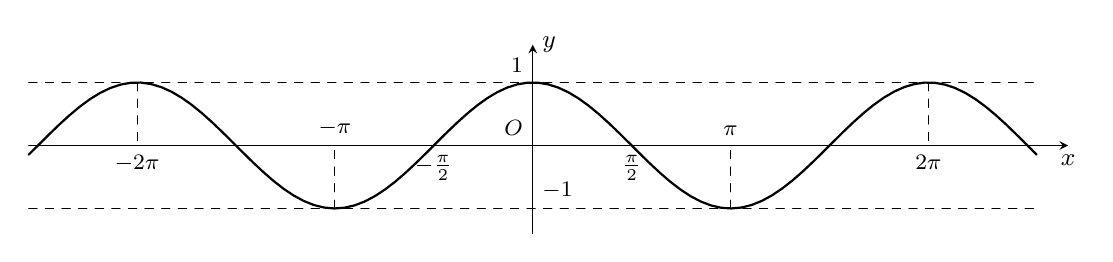
\begin{tikzpicture}[>=stealth,line join=round,line cap=round,font=\footnotesize,scale=0.8]
			\draw[->] (-8,0) -- (8.5,0) node[below] {\small $x$};
			\draw[->] (0,-1.4) -- (0,1.6) node[right] {\small $y$};
			\draw[thick,samples=100,domain=-8:8] plot(\x,{cos((\x)*180/pi)});
			\draw (0,0) node [above left] {$O$};
			\draw (0,1) node [above left] {$1$};
			\draw (0,-1) node [above right] {$-1$};
			\draw[dashed] (-3.14,-1)--(-3.14,0) node[above] {$-\pi$};
			\draw[dashed] (3.14,-1)--(3.14,0) node[above] {$\pi$};
			\draw[dashed] (-6.28,1)--(-6.28,0) node[below] {$-2\pi$};
			\draw[dashed] (6.28,1)--(6.28,0) node[below] {$2\pi$};
			\draw[dashed] (-1.57,0) node[below] {$-\frac{\pi}{2}$};
			\draw[dashed] (1.57,0) node[below] {$\frac{\pi}{2}$};
			\draw[dashed] (-8,1)--(8,1);
			\draw[dashed] (-8,-1)--(8,-1);
		\end{tikzpicture}
	\end{center}
	 Xét tính đúng sai của các khẳng định sau:
	 \choiceTF
	  {Hàm số đồng biến trên khoảng $(-\pi;\pi)$}
	 {\True Hàm số nghịch biến trên khoảng $(-2\pi;-\pi)$}
	 {\True Trên đoạn $[-2 \pi ; 2 \pi]$, hàm số có giá trị lớn nhất bằng 1}
	 {\True Trên đoạn $[-2 \pi ; 2 \pi]$, có đúng 3 giá trị của $x$ để hàm số nhận giá trị bằng $0$}
	 \loigiai{
	 }
\end{ex}

\begin{ex}%[1D1B4-6]
	Cho hàm số $y=\cot x$ có đồ thị như hình bên dưới.  
	\begin{center}
		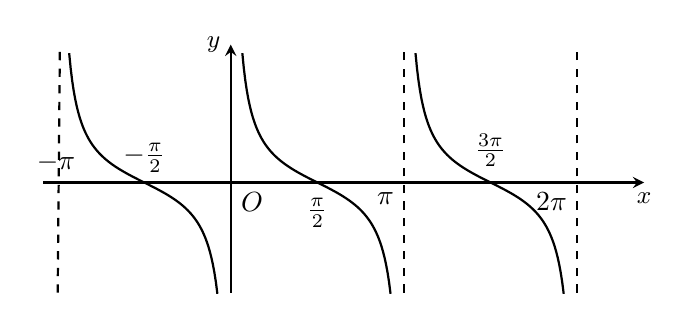
\begin{tikzpicture}[thick,>=stealth,scale=0.7,yscale=.5] 
			\draw[->] (-3.4,0) -- (7.5,0) node[below] {\small $x$};
			\draw[->] (0,-4) -- (0,5) node[left] {\small $y$};
			\draw (0,0) node[below right] {$O$};
			\draw[thick,samples=100,domain=0.21:2.9] plot(\x,{cot((\x)*180/pi)});
			\draw[thick,samples=100,domain=0.21:2.9] plot(\x-pi,{cot((\x)*180/pi)});
			\draw[thick,samples=100,domain=0.21:2.9] plot(\x+pi,{cot((\x)*180/pi)});
			%\draw[thick,samples=100,domain=0.21:2.9] plot(\x-2*pi,{cot((\x)*180/pi)});
			\draw (-3.17,0) node[above] {$-\pi$};
			\draw (3.14,0) node[below left=-0.1] {$\pi$};
			\draw (6.28,0) node[below left=-0.1] {$2\pi$};
			\draw (-1.57,0) node[above] {$-\frac{\pi}{2}$};
			\draw (1.57,-0.2) node[below] {$\frac{\pi}{2}$};
			%\draw (-4.71,-0.2) node[below] {$-\frac{3\pi}{2}$};
			\draw (4.71,0.2) node[above] {$\frac{3\pi}{2}$};
			\draw[dashed] (3.14,-4)--(3.14,5);
			\draw[dashed] (-3.14,-4)--(-3.1,5);
			\draw[dashed] (6.28,-4)--(6.28,5);
			%\draw[dashed] (-6.28,-4)--(-6.28,5);
		\end{tikzpicture}
	\end{center}
Xét tính đúng sai của các khẳng định sau:
\choiceTF
{\True Tập xác định của hàm số là $\mathbb{R}\setminus \left\{k\pi, k\in \mathbb{Z}\right\}.$}
{Hàm số nghịch biến trên $(-\pi;pi)$}
{Trên $[-\pi;\pi]$ có đúng ba giá trị của $x$ để $\cot x =0$}
{\True Trên $[0;\pi]$, $\cot x <1$ khi và chỉ khi $x \in \left(\dfrac{\pi}{4};\pi \right)$}
	\loigiai{
	}
\end{ex}

\begin{ex}
	Cho hàm số $y=f(x)=2\sin^2x-5$. Xét tính đúng sai của các khẳng định sau:
	\choiceTF
	{Hàm số tuần hoàn với chu kì $2\pi$}
	{\True Hàm số là một hàm số chẵn}
	{\True Giá trị lớn nhất của hàm số đạt được khi $x=\dfrac{\pi}{2}+k\pi$, với $k \in \mathbb{Z}$}
	{Giá trị nhỏ nhất của hàm số bằng $-3$}
	\loigiai{
	\begin{itemchoice}
		\itemch Hàm số tuần hoàn với chu kì $\pi$.
		\itemch Với mỗi $x \in \mathbb{R}$ thì 
		$f(-x)=2\sin^2(-x)-5=2\sin^2x-5$ nên hàm số đã cho là hàm số chẵn.
		\itemch Ta có $0 \le \sin^2 x \le 1 \Rightarrow =-5 \le 2\sin^2x-5 \le -3$. \\
		Suy ra, giá trị lớn nhất của hàm số bằng $-3$, đạt được khi $\sin^2 x =1 \Leftrightarrow \cos x =0 \Leftrightarrow x=\dfrac{\pi}{2}+k\pi$, với $k \in \mathbb{Z}$.
		\itemch Ta có $0 \le \sin^2 x \le 1 \Rightarrow =-5 \le 2\sin^2x-5 \le -3$. \\
		Suy ra, giá trị nhỏ nhất của hàm số bằng $-5$
\end{itemchoice}}
\end{ex}

\begin{ex}%[1D1B4-4]%[1D1T4-5]
	Huyết áp là áp lực máu cần thiết tác động lên thành động mạch nhằm đưa máu đi nuôi dưỡng các mô trong cơ thể. Nhờ lực co bóp của tim và sức cản của động mạch mà huyết áp được tạo ra. Giả sử huyết áp của một người thay đổi theo thời gian được cho bởi công thức:
	$p\left(t\right)=120+15\cos 150\pi t$,
	trong đó $p\left(t\right)$ là huyết áp tính theo đơn vị $\mathrm{mmHg}$ (milimét thủy ngân) và thời gian $t$ tính theo đơn vị phút.  Xét tính đúng sai của các khẳng định sau:
	\choiceTF
	{Hàm số $p(t)$ tuần hoàn với chu kì $\dfrac{\pi}{75}$}
	{Thời điểm $t=0$, huyết áp của người này là 120 $\mathrm{mmHg}$}
	{\True Huyết áp tâm thu (huyết áp cao nhất) của người này là $135$ $\mathrm{mmHg}$}
	{\True Huyết áp tâm tương (huyết áp thấp nhất) của người này là $105$ $\mathrm{mmHg}$}
	\loigiai{
		\begin{itemchoice}
			\itemch Ghi nhớ: Hàm số $y=\cos at$ tuần hoàn với chu kì $\dfrac{2\pi}{a}$. \\
			Suy ra hàm số này tuần hoàn với chu kì $\dfrac{2\pi}{150\pi}=\dfrac{1}{75}$.
			\itemch Với $t=0$, ta có $p=120+15 \cos 0 = 135$ $\mathrm{mmHg}$.
			\itemch Vì $-1\leq\cos 150\pi t\leq 1$ với mọi $t\in\mathbb{R}$ nên $105\leq p\left(t\right)\leq 135$ với mọi $t\in\mathbb{R}$ nên huyết áp tâm thu (huyết áp cao nhất) là $135$ $\mathrm{mmHg}$.
			\itemch Huyết áp tâm tương (huyết áp thấp nhất) của người này là $105$ $\mathrm{mmHg}$.
		\end{itemchoice}
	}
\end{ex}

\Closesolutionfile{ans}

\TNSA
\Opensolutionfile{ans}[ans/1D1-B3-3]

\begin{ex}
	Tìm giá trị lớn nhất của hàm số $y=\sqrt{5}-\sqrt{3}\cos 2x$. (Kết quả làm tròn đến hai chữ số thập phân)\\
	\shortans[oly]{$3,97$}
	\loigiai{
	Ta có $-1\le \cos 2x \le 1 \Rightarrow \sqrt{3}\ge -\sqrt{3}\cos 2x \ge -\sqrt{3} \Rightarrow \sqrt{5}+\sqrt{3}\ge \sqrt{5}-\sqrt{3}\cos 2x \ge \sqrt{5}-\sqrt{3}$.\\
	Suy ra giá trị lớn nhất của hàm số là $\sqrt{5}+\sqrt{4} \approx 3,97.$
}
\end{ex}

\begin{ex}%[1D1B1-6]%
	Xét hàm số $f(x)=\cos 2x$ trên $[0;2\pi]$ có đồ thị như hình vẽ.
	\begin{center}
		\begin{tikzpicture}[>=stealth,x=1.3cm,y=1cm,scale=1]
			\draw[->] (-1,0) -- (7,0) node[below] {\small $x$};
			\draw[->] (0,-1.4) -- (0,1.4) node[right] {\small $y$};
			\draw [fill=white,draw=black] (0,0) circle (1pt)node[below left] {\footnotesize $O$};
			\draw[smooth,samples=100,domain=0:6.283] plot(\x,{cos((2*(\x))*180/pi)});
			\draw[dashed] (6.283,1)--(6.283,0) (3.142,1)--(3.142,0);
			\draw[fill=black] (0.785,0)node [below]{\footnotesize  $\dfrac{\pi}{4}$} circle(0.03);
			\draw[fill=black] (2.356,0)node [above]{\footnotesize  $\dfrac{3\pi}{4}$} circle(0.03);
			\draw[fill=black] (3.927,0)node [above]{\footnotesize  $\dfrac{5\pi}{4}$} circle(0.03);
			\draw[fill=black] (5.498,0)node [above]{\footnotesize  $\dfrac{7\pi}{4}$} circle(0.03);
			\draw[fill=black] (3.142,0)node [below]{\footnotesize  $\pi$} circle(0.03);
			\draw[fill=black] (6.283,0)node [below]{\footnotesize  $2\pi$} circle(0.03);
			\draw[fill=black] (0,1)node [left]{\footnotesize  $1$} circle(0.03);
		\end{tikzpicture}
	\end{center}
Gọi $T$ là tập hợp tất cả các giá trị của $x \in [0;2\pi]$ để $\cos 2 x =0$. Tính tổng tất cả các phần tử của $T$ (làm tròn đến hàng phần chục).\\
\shortans[oly]{$12,6$}
	\loigiai{
		Dựa vào đồ thị $T=\left\{\dfrac{\pi}{4};\dfrac{3\pi}{4};\dfrac{5\pi}{4};\dfrac{7\pi}{4}\right\}$. Suy ra, tổng các phần tử trong tập hợp $T$ là 
		$$\dfrac{\pi}{4}+\dfrac{3\pi}{4}+\dfrac{5\pi}{4}+\dfrac{7\pi}{4} \approx 12,6.$$
	}
\end{ex}

\begin{ex}%Câu 1.24.%[1D1V4-8] 
	Hằng ngày, Mặt Trời chiếu sáng, bóng của một tòa chung cư cao $40\,\mathrm{(m)}$ in trên mặt đất, độ dài bóng của tòa nhà này được tính bằng công thức
	$S\left( t \right)=40\left| \cot\dfrac{\pi }{12}t \right|$,
	ở đó $S$ được tính bằng mét, còn $t$ là số giờ tính từ $6$ giờ sáng. Tìm độ dài bóng của tòa nhà tại các thời điểm $8$ giờ sáng (làm tròn đến hàng phần chục).\\
	\shortans[oly]{$169,3$}
	\loigiai{Tại thời điểm $8$ giờ sáng ta có $t=8-6=2$. \\
		Vậy độ dài bóng của tòa nhà tại thời điểm $8$ giờ sáng là
		$S\left( 2 \right)=40\left| \cot\left( \dfrac{\pi }{12}\cdot 2 \right) \right|=40\sqrt{3}\,\mathrm{(m)}$
	}	
\end{ex}

\begin{ex}%[Tex hóa SGK 11, KNTT]%[Phạm Tuấn]%[1K1B3-5] 
	Giả sử khi một cơn sóng biển đi qua một cái cọc ở ngoài khơi, chiều cao của nước được mô hình hoá bởi hàm số $h(t)=90 \cos \left(\dfrac{\pi}{10} t\right)$, trong đó $h(t)$ là độ cao tính bằng centimét trên mực nước biển trung bình tại thời điểm $t$ giây. Tìm chiều cao của sóng (cm) (là khoảng cách theo phương thẳng đứng giữa đáy và đỉnh của sóng).\\
	\shortans[oly]{$180$}
	\loigiai{
		Ta có $-90 \leq 90 \cos \left(\dfrac{\pi}{10} t\right) \leq 90$, suy ra chiều cao của sóng là $90- (-90) =180$ (cm).	}
\end{ex}


\begin{ex}%[Thi thử L2, Chuyên DHSP Ha Noi, 2018 ]%[1D1K1-6]%[MyNguyen, Dự án (12EX-8)]
	\immini[thm]{Cho hai điểm $A$, $B$ thuộc đồ thị hàm số $y=\sin x$ trên đoạn $[0;\pi]$, các điểm $C$, $D$ thuộc trục $Ox$ thỏa mãn $ABCD$ là hình chữ nhật và $CD=\dfrac{2\pi}{3}$. Tính độ dài đoạn $BC$.\\
		\shortans[oly]{$0,5$}
		}{\hspace{0.4cm}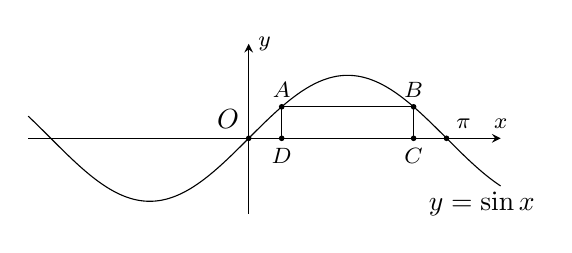
\begin{tikzpicture}[>=stealth,x=1.0cm,y=1.0cm, scale=0.8]
			\draw[->](-3.5,0) -- (4,0) node[above]{\footnotesize $x$};
			\draw[->](0,-1.2) -- (0,1.5) node[right]{\footnotesize $y$};
			\draw[fill=black] (0,0) node [above left]{$O$} circle (1pt);
			\draw[fill=black] (3.14,0) node [above right]{\footnotesize $\pi$} circle (1pt);
			\draw[smooth, samples=100, domain=-3.5:4]plot(\x,{sin((\x)*180/pi)});
			\draw (pi/6,0)--(pi/6,0.5)--(5*pi/6,0.5)--(5*pi/6,0);
			\draw[fill=black] (pi/6,0) node [below]{\footnotesize $D$} circle (1pt);
			\draw[fill=black](pi/6,0.5) node [above]{\footnotesize $A$} circle (1pt);
			\draw[fill=black] (5*pi/6,0.5) node [above]{\footnotesize $B$} circle (1pt);
			\draw[fill=black] (5*pi/6,0) node [below]{\footnotesize $C$} circle (1pt);
			\node at (3.7,-0.7) [below]{$y=\sin x$};
	\end{tikzpicture}}
	\loigiai{
		Theo hình vẽ thì $OD=CK \Rightarrow 2OD=\pi-CD=\dfrac{\pi}{3}\Rightarrow OD=\dfrac{\pi}{6}\Rightarrow x_D=\dfrac{\pi}{6}$.\\
		Tung độ điểm $D$ là $y_D=\sin\left(\dfrac{\pi}{6} \right)=\dfrac{1}{2}=AD=BC$. 
	}
\end{ex}


\Closesolutionfile{ans}



